\documentclass[a4paper,14pt]{extarticle}
\usepackage{cmap}				% To be able to copy-paste russian text from pdf			
\usepackage[utf8]{inputenc}
\usepackage[margin=1in]{geometry}
\usepackage[russian]{babel}
\usepackage{enumitem} % remove left identation from list environment
\usepackage{graphicx}
\usepackage{caption}
\usepackage{hyperref}

\usepackage[
	output-decimal-marker={,},
	group-separator={\,},
	group-minimum-digits=3
]{siunitx}

\newcommand{\foreign}[1]{\textit{#1}}
\newcommand{\english}[1]{#1}

\author{Артём Бакулин}
\date{30 июля 2019 г.}
\title{Валютный рынок и финансовая инженерия в Средние века}

\begin{document}

\maketitle

\begin{figure}[h]
\centering
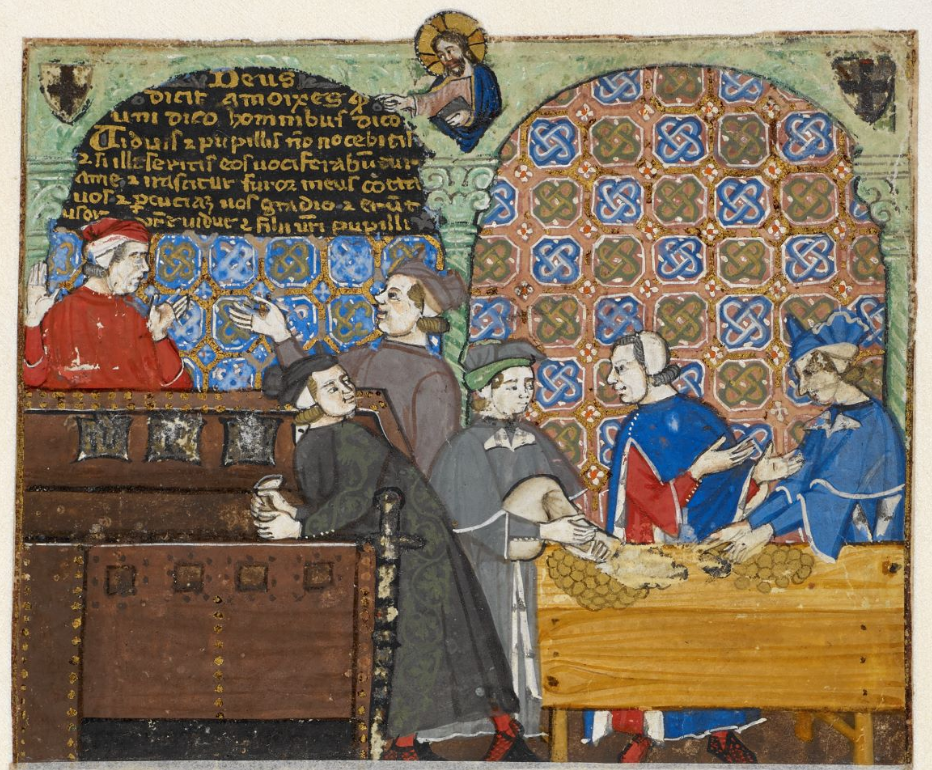
\includegraphics[scale=0.5]{avarice.png}
\captionsetup{labelformat=empty}
\caption{<<Алчность>>. Миниатюра из манускрипта. Генуя, ок. 1330 г., Британская библиотека.
URL: \url{http://www.bl.uk/manuscripts/FullDisplay.aspx?ref=Add_MS_27695}}
\end{figure}

\section*{Грех ростовщичества и банковское дело}

Как известно, в Средние века Римско-католическая церковь не очень-то жаловала ростовщиков. В наказание за грех ростовщичества можно было схлопотать отлучение от церкви, что гарантировало попадание в ад после смерти. Согласно Данте, на седьмом круге ада ростовщиков (а также богохульников и содомитов) ожидали пустынные горючие пески и огненный дождь. Стоит отметить, что если сегодня мы обычно называем ростовщичеством взимание неоправданно высоких, грабительских, процентов, то в Средневековье Церковь считала грехом и карала за требование любой суммы сверх тела долга, даже самой ничтожной. В довесок грешником становился не только сам ростовщик, но и его должник, согласившийся выплачивать проценты.

Нужно ли говорить, что средневековые банкиры проявляли недюжинную изворотливость, чтобы кредитовать клиентов в таком неблагоприятном инвестиционном климате? К XIV веку коллективная мысль придумала сразу несколько уловок, чтобы обойти религиозный запрет.

Во-первых, Церковь не запрещала подарки. Клиент имел полное право от чистого сердца поблагодарить банкира за оказанную услугу, заплатив немного больше, чем тело кредита. Разумеется, клиент и банкир ни в коем случае не должны были загодя договариваться о точном размере подарка. Любопытно, что и банкиры могли делать подарки вкладчикам. Известно, что срочные депозиты в банках Флоренции приносили проценты \foreign{a discrezione}, то есть на усмотрение банкира, как жест доброй воли. Конечно, банкир, который недостаточно щедро выплачивал <<добровольные>> проценты, рано или поздно проигрывал конкурентам.

Во-вторых, Церковь дозволяла штрафы и возмещение убытков. Если клиент не успевал вернуть долг в срок, то он должен был заплатить штраф, так как банкир мог за время просрочки упустить возможность выгодно вложить деньги. Осталось только указать в договоре и в банковском гроссбухе одну дату погашения, пораньше, а на словах договориться о другой, попозже. Штрафы, накопившиеся за время воображаемой просрочки, станут замаскированной процентной ставкой. Поразительно, но мы слышим отголоски этой схемы едва ли не каждый день: английское слово \english{interest} происходит от средневекового латинского \foreign{interesse} (возмещение ущерба).

В-третьих, банкир мог скрыть истинный размер долга. В гроссбух он записывал сумму, равную будущей выплате, а на деле выдавал клиенту чуть меньше. Такое <<творческое>> ведение счетов опасно тем, что требует махинаций не только в записях банкира, но и в бухгалтерии клиента, у которого может не сойтись баланс. Тем не менее, исследователи обнаружили следы подтасовок даже в документах английского королевского казначейства (\english{the Exchequer}): в XIII--XIV веках английские монархи, начиная с  Эдуарда I, часто пользовались услугами итальянских банков.

Наконец, в-четвёртых, банкиры научились использовать валютный рынок, чтобы создавать синтетические кредиты, прямо как заправские финансовые инженеры с PhD и MBA. Этот способ мы и рассмотрим ниже.

\section*{Средневековый валютный рынок}
Основным инструментом валютных трейдеров XIV века был вексель или, проще говоря, расписка (\english{bill of exchange}). По расписке можно было получить валюту в одном городе, а расплатиться второй валютой в другом городе через фиксированный срок. Срок выплаты во втором городе обычно зависел от расстояния. Скажем, для сделок между Флоренцией и Венецией стандартный срок составлял 10 дней, а для сделок между Венецией и Лондоном --- три месяца.

Рассмотрим пример. Если некий купец собирался купить товары в Венеции и продать их в Лондоне, то он мог прийти в венецианский банк и попросить 100 венецианских дукатов. Взамен купец давал банкиру расписку, по которой тот мог получить в лондонском банке 20 фунтов через 3 месяца. Купца ещё называли продавцом расписки, а банкира --- покупателем, потому что в день сделки банкир <<покупал>> у купца расписку за живые деньги. Говоря современным языком, банкир покупал валютную пару GBPDUC по курсу 5 дукатов сегодня за 1 фунт через три месяца. Однако, в отличие от современных валютных сделок, обмен был растянут во времени. Все три месяца банкир должен был терпеливо ждать и надеяться, что продавец благополучно доберётся до Лондона и выполнит свои обязательства.

Если всё шло хорошо, то трёх месяцев было вполне достаточно, чтобы купец приобрёл товары в Венеции за дукаты, прибыл с ними в Лондон, продал за фунты и внёс в местный банк необходимые 20 фунтов. Тем временем банкир отправлял своему лондонскому коллеге саму расписку. Получив расписку и деньги, лондонский банкир переносил фунты со счёта купца на счёт венецианского банкира, и все оставались довольны. Церковь не возражала против такой транзакции, следуя принципу \foreign{cambium non est mutuum} (обмен --- не долг).

\section*{Финансовая инженерия XIV века}
Как быть, если купец не смог собрать 20 фунтов к оговоренному сроку или вообще не появился в Лондоне? Лондонский банк имел право <<опротестовать>> расписку, то есть принудительно заключить обратную сделку между венецианским банкиром и купцом от их имени. В этой новой сделке купец получал недостающие 20 фунтов, а расплачивался распиской на получение дукатов ещё через 3 месяца. Например, если к моменту заключения обратной сделки (через три месяца после сделки в Венеции) рыночный курс в Лондоне составлял \num{5.3} дуката за 1 фунт, то купец был обязан заплатить венецианскому банкиру 106 дукатов ещё через три месяца. Другими словами, лондонский банк ничем не рисковал и предлагал венецианскому банкиру самостоятельно разобраться со своим незадачливым клиентом.
\begin{table}[h]
\centering
\begin{tabular}{l|l|l}
Дата & Прямая сделка & Обратная сделка \\ \hline
0 мес. & +100 дукатов & \\
3 мес. & --20 фунтов & +20 фунтов \\
6 мес. & & --106 дукатов
\end{tabular}
\captionsetup{labelformat=empty}
\caption{Платежи купца в результате прямой и обратной сделок.}
\end{table}

Звучит сложновато, но нам важно проследить суммарный эффект прямой и обратной сделок. Что называется, следите за руками. Купец получил 100 дукатов в банке в Венеции, а через полгода заплатил тому же банку 106 дукатов в Венеции. Платежей в фунтах как не бывало, они схлопнулись в ноль. Более того, совершенно не обязательно было покупать товары и тащиться за тридевять земель в промозглый Лондон, ведь английский банк мог запустить процесс опротестования расписки самостоятельно. Гораздо приятнее остаться в солнечной Италии и пустить 100 дукатов на развитие бизнеса в Венеции. Что это, как не кредит под 12\% годовых? Так две разрешённые Церковью валютные сделки лёгким движением руки превратились в запрещённый кредит.

Строго говоря, двойная сделка с валютой не является кредитом под фиксированную ставку. Процент, который заработает банкир, зависит от того, по какому курсу удастся заключить вторую сделку в Лондоне. Если за эти три месяца случится средневековый Брекзит, и фунт просядет до 4 дукатов за фунт, то банкир не только не заработает, но ещё и потеряет 20 дукатов. Неопределённость будущей прибыли, кстати, была важным аргументом в споре о греховности двойных валютных сделок. Какое ростовщичество, уважаемая Церковь, если клиент потенциально мог вернуть меньше, чем одолжил?!

Конечно, банкир должен был закладывать валютный риск в самую первую сделку. Уже тогда люди понимали, что деньги сейчас и деньги через три месяца --- это не одно и то же. Например, если рыночный курс фунта к дукату при обмене монета на монету составлял \num{5.15} дуката за фунт, то в Венеции банкиры покупали расписки на будущие фунты по \num{5.0} (чуть дешевле), а в Лондоне продавали фунты за будущие дукаты по \num{5.3} (чуть дороже). Очень похоже на современные обменники с их широченным спрэдом между курсами покупки и продажи, не правда ли?

Чтобы оставаться конкурентоспособными на валютном рынке, все --- и банкиры, и купцы --- нуждались в актуальной информации о валютных курсах во всех крупных городах. Считалось хорошим тоном в конце каждого делового письма добавить последние котировки местного валютного рынка. Сохранившиеся с тех времён письма позволили учёным составить достаточно длинные временные ряды валютных курсов в главных финансовых центрах Европы, а также оценить доходность кредитов, созданных из валютных сделок.

Выяснилось, что разность между курсами покупки и продажи позволяла банкирам зарабатывать 10--16\% годовых, какие бы два города ни участвовали в сделке --- что Флоренция и Венеция (в среднем \num{10.9}\% годовых, 30 дней на две сделки), что Генуя и Лондон (в среднем \num{14.5}\% годовых, 180 дней на две сделки). Конечно, случались и потери, но на длинной дистанции стратегия работала. Для сравнения, в тот же период аренда земли в Италии приносила 8--10\% годовых, а флорентийские депозиты \foreign{a discrezione} --- от 6\% до 10\%. Есть свидетельства, что банк Медичи просил 10--12\% годовых за кредиты, полностью обеспеченные залогом. Поэтому упомянутые 10--16\% годовых выглядят вполне разумной ставкой для необеспеченного кредита, который к тому же несёт валютный риск.

Мы не знаем наверняка, какая часть валютных сделок использовалась для создания кредитов. Далеко не все расписки проходили процедуру опротестования, к тому же обычно записи в банковских книгах не отвечают на вопрос, по какой причине продавец не смог выполнить свои обязательства. Может быть, он потерял груз в шторме, а может быть, это была часть устного договора с банкиром. С другой стороны, сохранились свидетельства и полностью искусственных сделок, когда банкир даже не заморачивался с отправкой расписок в другой город, а просто заносил в свои книги прямую и обратную сделку по выдуманным им курсам. Скорее всего, в большинстве случаев купцы использовали валютный рынок по назначению, для международной торговли, и лишь иногда для того, чтобы взять кредит.

\section*{Заключение}
Я затрудняюсь сформулировать личное отношение ко всему, о чём рассказал вам. С одной стороны, изобретательность --- прекрасное качество. Особенное восхищение вызывает то, что эти господа проворачивали сделки, когда на кону стояли не штрафы и годы в тюрьме, а бессмертные души и вечные адские муки. С другой стороны, я погружаюсь в грустные мысли о природе человека. Выходит, что возможность злоупотреблений --- неизбежная обратная сторона финансовых инноваций и экономического роста.

\section*{Ссылки}

\begin{enumerate}[leftmargin=*]
\item Bell, Adrian R., Chris Brooks, and Tony K. Moore. ``Cambium non est mutuum: exchange and interest rates in medieval Europe.'' \textit{The Economic History Review} 70.2 (2017): 373--396. URL: \url{http://centaur.reading.ac.uk/57199/1/Bell_Brooks_Moore_cambium_not_est_mutuum.pdf}

\item Bell, Adrian R., Chris Brooks, and Tony K. Moore. ``Interest in medieval accounts: examples from England, 1272–1340.'' \textit{History} 94.316 (2009): 411--433. URL: \url{http://centaur.reading.ac.uk/16784/1/16784.pdf}

\item Goldthwaite, Richard A. ``Local banking in renaissance Florence.'' \textit{Journal of European Economic History} 14.1 (1985): 5--55. URL: \url{http://www.jeeh.it/articolo?urn=urn:abi:abi:RIV.JOU:1985;1.5&ev=1}

\item Alighieri, Dante. \textit{La Comedia di Dante Alleghieri}. Johann Numeister and Evangelista Angelini da Trevi, 1472.
\end{enumerate}


\end{document}